\documentclass[conference]{IEEEtran}
\usepackage[utf8]{inputenc}
\usepackage[spanish]{babel}
\usepackage{graphicx}
\usepackage{url}
\usepackage{cite}
\usepackage{apacite}


\title{Desarrollo de un Chatbot Experto en Vinos Usando la API Moderna de OpenAI y Tkinter}
\author{\IEEEauthorblockN{Roberto Alvarado}
\IEEEauthorblockA{UTPL
Email: raalvarado6@utpl.edu.ec}}

\begin{document}

\maketitle

\begin{abstract}
Este trabajo presenta el desarrollo de un chatbot experto en vinos. Se diseñó
una interfaz gráfica con Tkinter en Python para facilitar la interacción con el
usuario. Además, se creó un conjunto de datos en formato CSV con 20 vinos, sus
características y precios imaginarios, que se utilizan como contexto para las
respuestas del chatbot. Se implementó un modo de prueba automática para validar
el desempeño del modelo en preguntas frecuentes. También se describen las
buenas prácticas para proteger la clave API y la organización del proyecto para
su publicación en GitHub.
\end{abstract}

\begin{IEEEkeywords}
chatbot, OpenAI, GPT-4, Tkinter, vinos, inteligencia artificial, API, CSV,
pruebas automáticas
\end{IEEEkeywords}

\section{Introducción}
El uso de chatbots en la acutalidad se ha consolidado como una herramienta clave en diversos
ámbitos, permitiendo la automatización de la comunicación con los usuarios para
ofrecer información y asistencia de manera eficiente. En este proyecto se
presenta el desarrollo de un chatbot especializado en el dominio del vino,
diseñado para responder preguntas con base en una base de datos estructurada y
enriquecida. Para ello, se aprovechan las capacidades avanzadas de los modelos
de lenguaje de última generación, como GPT-3.5 de OpenAI. Asimismo, se incorpora
una interfaz gráfica desarrollada en Python, con el objetivo de ofrecer una
experiencia de usuario clara, intuitiva y accesible.

\section{Marco Teórico}
Los chatbots se pueden dividir según su arquitectura y qué tipo de
información manejan. Algunos funcionan con reglas fijas, por lo que solo pueden
dar respuestas limitadas, pero siempre responden de forma predecible. Otros,
como los que usan inteligencia artificial y modelos como GPT-4, aprenden del
lenguaje y pueden dar respuestas más completas y adaptadas a cada situación.
\cite{shawar2007chatbots,adamopoulou2020overview}. La API de OpenAI provee
acceso a modelos de lenguaje con capacidad para entender y generar
texto natural \cite{brown2020language}.

Tkinter es un toolkit estándar para crear interfaces gráficas en Python,
permitiendo un desarrollo rápido y multiplataforma \cite{lundh2001python}.
¿Por qué no se utilizo un sistema web? Algo que no se considera frecuentemente
en la actualidad es el consumo de recursos y de tokens,
para este experimento se decidió utilizar tkinter para tener un sistema
local. Y que no tiene finalidad en la web. Se puede mejorar pero cumple la misma
funcionalidad


\section{Trabajos Relacionados}
Muchos estudios han explorado chatbots especializados en áreas como salud,
educación y gastronomía. Por ejemplo, chatbots para asesoría en vinos han sido
desarrollados con bases de datos estáticas y reglas predefinidas
\cite{vinbot2019}. La integración de modelos de lenguaje avanzados con bases de
datos personalizadas representa una evolución que mejora la naturalidad y
precisión de las respuestas.

\section{Metodología}

\subsection{Definición del Alcance}
El chatbot está diseñado para responder preguntas relacionadas con 20 vinos
representativos, detallando año, tipo de uva, maridaje, origen y precio. El
dominio se limita a esta base para garantizar respuestas precisas y
especializadas.

\subsection{Recolección de Datos}
Se creó un archivo CSV con la siguiente estructura:

nombre,año,uva,maridaje,origen,precio\_usd

\subsection{Diseño y Desarrollo}

Se utilizó
\begin{itemize}
    \item \textbf{OpenAI API:} Uso de la clase \texttt{OpenAI} para gestionar llamadas a GPT-4.
    \item \textbf{Tkinter:} Para interfaz gráfica de chat.
    \item \textbf{pandas:} Lectura y procesamiento del CSV.
    \item \textbf{python-dotenv:} Gestión segura de variables de entorno para la API Key.
\end{itemize}

El contexto con la información del CSV se prepara concatenando los datos y
limitando el tamaño para evitar exceder los límites de tokens. El chatbot
responde exclusivamente en base a esta información.


\subsection{Protocolo Conversacional}

El chatbot inicia con un mensaje de bienvenida, y las preguntas del usuario se
envían al modelo junto con el contexto. La respuesta se muestra en la interfaz
en formato conversación. Para setear el chatbot lo que hice fue utilizar
un preambulo o contexto para explicarle como responder, este fue el preambulo

\textit{
Eres un sommelier experto en vinos. Si preguntan sobre alguna recomendación,
intenta primero explicar de manera general en base a tu conocimiento de vinos,
y después has una recomendación, por favor dame el vino en una sola linea con
el precio, y el origen, junto a su año y el tipo de vua. Estos son los vinos
que tengo en mi stock, si preguntan sobre recomendaciones utiliza este
stock:+ <CSV\_CONTEXT>}

Algo importante, que se aumento es que durante la conversación cada
pregunta se va guardando para que el chatbot tenga contexto

\subsection{Pruebas Automáticas}

Se implementó un modo de test ejecutable con el parámetro \texttt{--test} que
realiza 5 preguntas frecuentes sobre vinos y muestra las respuestas en consola
para validar la coherencia y pertinencia.

\subsection{Seguridad y Buenas Prácticas}

La clave API se almacena en un archivo \texttt{.env}, nunca incluido en
repositorios públicos. Se recomienda usar archivos \texttt{.gitignore} para
evitar subir claves por error.

Para que el programa para que pueda ser utilizado por el profesor, sin la necesidad
de una APIKEY,
cree una sistema de cifrado que codifica el api\_key con una clave que le enviaré personalmente
para que pueda utilizarlo


\section{Repositorio y Ejecución del Programa}

El código fuente completo de este proyecto está disponible en el siguiente repositorio de GitHub:

\begin{center}
\textbf{\url{https://github.com/Robdres/TAF_vinos/}}
\end{center}

\subsection{Requisitos previos}

\begin{itemize}
    \item Python 3.9 o superior.
    \item Una cuenta activa de OpenAI con acceso a la API, a menos de tener
        la clave
\end{itemize}

\subsection{Instrucciones de instalación y ejecución}

\begin{enumerate}
    \item Clonar el repositorio:
    \begin{verbatim}
git clone https://github.com/
    Robdres/TAF_vinos/
cd TAF_vino
    \end{verbatim}

    \item Instalar las dependencias:
    \begin{verbatim}
pip install -r requirements.txt
    \end{verbatim}

    \item Si quiere utilizar su propia OpenAI puede
        create un .env file en el mismo archivo que tenga
        como argumento
    \begin{verbatim}
OPENAI_API_KEY="<su-api-key>"
    \end{verbatim}

    \item Ejecutar la aplicación principal con interfaz gráfica (Tkinter):
    \begin{verbatim}
python main.py
    \end{verbatim}


    \item Ejecutar el modo de prueba automática:
    \begin{verbatim}
python main.py --test
    \end{verbatim}

    \item Si no tiene su propia key, se le pedirá una clave
        ingresela y puede continuar

\end{enumerate}
\section{Resultados}
En la figura 1 podemos ver la interfaz y una pregunta.
En la figura 2 podemos ver que tiene el contexto de las anteriores preguntas
\begin{figure}[htbp]
\centerline{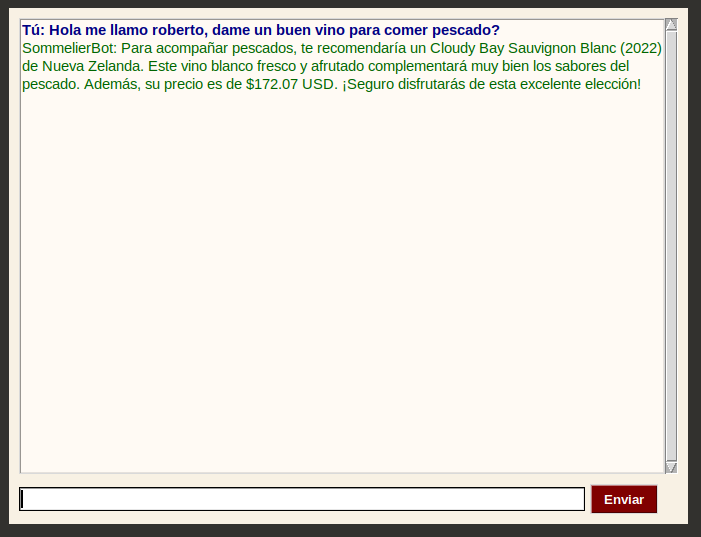
\includegraphics[width=0.48\textwidth]{./figures/2025-06-01-100101_701x537_scrot.png}}
\caption{Captura de pantalla de la interfaz Tkinter del chatbot sommelier.}
\label{fig:interfaz}
\end{figure}

\begin{figure}[ht]
\centerline{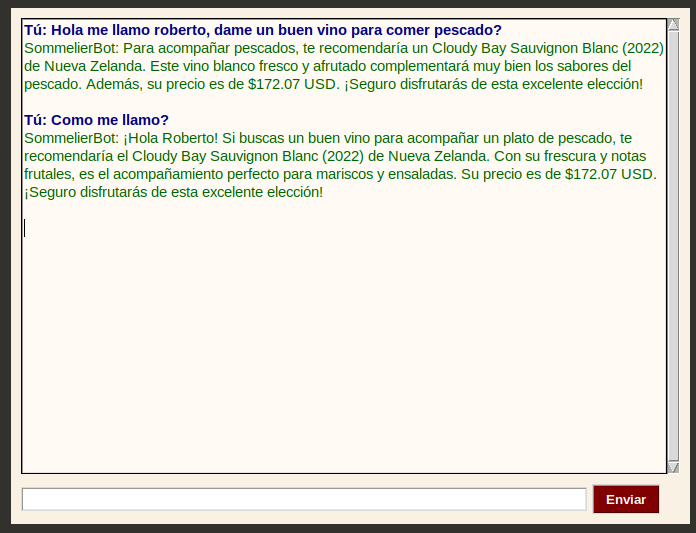
\includegraphics[width=0.48\textwidth]{./figures/2025-06-01-100135_696x533_scrot.png}}
\caption{Captura de pantalla de la interfaz Tkinter del chatbot sommelier.}
\label{memory}
\end{figure}

Las pruebas automáticas mostraron respuestas coherentes y basadas en la base de
datos, confirmando la correcta integración del modelo y el procesamiento del
CSV.

Para los resultado del testing, por favor ver el appendice con los resultados
de las respuestas que validan que el chatbot esta funcionando

\section{Conclusiones}

Se desarrolló exitosamente un chatbot experto en vinos que utiliza la última
versión de la API de OpenAI con la clase \texttt{OpenAI}, integrando una base
de datos en CSV y una interfaz gráfica con Tkinter. El sistema cuenta con un
modo de pruebas automáticas para validar respuestas. Se documentaron buenas
prácticas para la protección de la clave API y la organización para la
publicación en GitHub.

\section*{Apendice: Resultados del testing}
- Test 1: ¿Qué vino va bien con carne de cerdo?

- Para maridar con carne de cerdo, te recomendaría un vino con buena acidez y cuerpo medio que complemente los sabores de la carne sin opacarla. En este caso, un Riesling alemán sería una excelente elección, ya que su acidez equilibrada y notas frutales pueden realzar los sabores del cerdo sin dominarlos. ¡Te recomiendo el Mosel Riesling Spätlese (2021) de Alemania, con un precio de \$278.86 USD!
\vspace{0.1cm}
\hrule
\vspace{0.1cm}
- Test 2: ¿Cuál es el vino más barato de la lista?

- Para maridar con carne de cerdo, te recomendaría un vino con buena acidez y cuerpo medio que complemente los sabores de la carne sin opacarlos. En este caso, te sugiero el Mosel Riesling Spätlese (2021) de Alemania, elaborado con uva Riesling, que tiene notas frutales y una acidez refrescante que armoniza muy bien con la carne de cerdo. Además, su precio es de \$278.86 USD.
El vino más barato de la lista es el Dom Pérignon (2013) de Francia, elaborado con uvas Chardonnay y Pinot Noir, ideal para maridar con caviar u ostras, y tiene un precio de \$22.51 USD. ¡Una excelente opción para disfrutar de un champagne de alta calidad a un precio accesible!
\vspace{0.1cm}
\hrule
\vspace{0.1cm}
- Test 3: ¿Tienes un vino argentino?

- ¡Claro! Los vinos argentinos suelen ser reconocidos por su calidad, especialmente aquellos elaborados con la uva Malbec. En este caso, te recomendaría el **Catena Zapata Adrianna (2018)**, un vino argentino excepcional elaborado con uva Malbec, ideal para maridar con carnes asadas y quesos fuertes.
Precio: \$39.95 USD - Origen: Argentina - Año: 2018 - Uva: Malbec
\vspace{0.1cm}
\hrule
\vspace{0.1cm}
- Test 4: Dime un vino con uva Malbec

- El vino argentino Catena Zapata Adrianna (2018) es una excelente opción, ya que está elaborado con uva Malbec, la cual es bastante característica de Argentina. Este vino marida muy bien con carnes asadas y quesos fuertes. Su precio es de \$39.95 USD.
\vspace{0.1cm}
\hrule
\vspace{0.1cm}
-- Test 5: ¿Cuál recomiendas con pescado?

-- Para maridar con carne de cerdo, te recomendaría buscar un vino tinto con buena acidez, como un Pinot Noir o un Tempranillo joven.
El vino más barato de la lista es el Dom Pérignon (2013) con un precio de \$22.51 USD.
¡Claro que sí! Tenemos un vino argentino en la lista que es el Catena Zapata Adrianna (2018), elaborado con uva Malbec.
Un excelente vino con uva Malbec que te recomendaría es el Catena Zapata Adrianna (2018) de Argentina, ideal para maridar con carnes asadas y quesos fuertes.
Si estás buscando un vino para maridar con pescado, te recomendaría el Chablis Grand Cru (2021) de Francia, elaborado con uva Chardonnay y perfecto para acompañar pescados blancos y mariscos. Su precio es de \$217.06 USD.


\bibliographystyle{apacite}
\bibliography{referencias}

\end{document}

